\documentclass[9pt,a4paper]{article}

\usepackage[margin=1.2cm, top=0.8cm, bottom=0.8cm]{geometry}
\usepackage[dvipsnames,table]{xcolor}
\usepackage{tikz}
\usepackage[T1]{fontenc}
\usepackage{enumitem}
\usepackage{tabularx}
\usepackage{booktabs}
\usepackage{multicol}
\usepackage{fancyhdr}
\usepackage{hyperref}
\usepackage{sourcecodepro}
\usepackage{microtype}
\usepackage{titlesec}
\usepackage{parskip}

% ── Colors ────────────────────────────────────────────────
\definecolor{molpurple}{HTML}{7C3AED}
\definecolor{molpink}{HTML}{EC4899}
\definecolor{moldark}{HTML}{1E1B2E}
\definecolor{molgray}{HTML}{6B7280}
\definecolor{mollight}{HTML}{F5F3FF}
\definecolor{molgreen}{HTML}{10B981}
\definecolor{molorange}{HTML}{F59E0B}
\definecolor{molblue}{HTML}{3B82F6}

\hypersetup{colorlinks=true, linkcolor=molpurple, urlcolor=molpurple, pdftitle={MOL Language}, pdfauthor={CruxLabx}}

\titleformat{\section}{\normalsize\bfseries\color{molpurple}}{}{0em}{}[\vspace{-0.4em}\textcolor{molpurple}{\rule{\linewidth}{0.3pt}}]
\titlespacing{\section}{0pt}{0.35em}{0.1em}

\pagestyle{fancy}
\fancyhf{}
\renewcommand{\headrulewidth}{0pt}
\fancyfoot[L]{\scriptsize\color{molgray}\textcopyright\ 2026 CruxLabx / IntraMind. All rights reserved.}
\fancyfoot[R]{\scriptsize\color{molgray}\url{github.com/crux-ecosystem/mol-lang}}

\setlist[itemize]{nosep, leftmargin=1em, label=\textcolor{molpurple}{\textbullet}}
\newcommand{\code}[1]{\texttt{\small\color{molpurple}#1}}
\newcommand{\badge}[2]{\tikz[baseline=(n.base)]{\node[fill=#1,rounded corners=2pt,inner sep=1.5pt,text=white,font=\sffamily\fontsize{5.5}{6}\selectfont\bfseries](n){#2};}}
\newcommand{\stat}[2]{\begin{center}\textcolor{molpurple}{\Large\bfseries #1}\\[-3pt]{\fontsize{6}{7}\selectfont\color{molgray}#2}\end{center}}

\begin{document}
\setlength{\parskip}{0pt}

% ── HEADER ────────────────────────────────────────────────
\begin{tikzpicture}[remember picture, overlay]
  \fill[moldark] (current page.north west) rectangle ([yshift=-2.4cm]current page.north east);
  \node[anchor=west, text=white, font=\fontsize{28}{32}\selectfont\bfseries\sffamily] at ([xshift=1.2cm, yshift=-0.9cm]current page.north west) {MOL};
  \node[anchor=west, text=molpink, font=\normalsize\sffamily] at ([xshift=4.8cm, yshift=-0.8cm]current page.north west) {The Cognitive Programming Language};
  \node[anchor=west, text=white!70, font=\scriptsize] at ([xshift=1.2cm, yshift=-1.55cm]current page.north west) {Native pipeline operators \textbar\ Auto-tracing \textbar\ AI domain types \textbar\ RAG built-in \textbar\ Transpiles to Python \& JS};
  \node[anchor=west, font=\scriptsize] at ([xshift=1.2cm, yshift=-2.05cm]current page.north west) {%
    \badge{molpurple}{v0.3.0}\;\badge{molgreen}{68 Tests}\;\badge{molorange}{90+ Functions}\;\badge{molblue}{Python 3.10+}\;\badge{molgray}{CruxLabx / IntraMind}%
  };
\end{tikzpicture}

\vspace{1.8cm}

% ── INTRO + STATS ─────────────────────────────────────────
{\small\textbf{MOL} is the first language with native \code{|>} pipeline operators and automatic execution tracing --- built for AI/RAG pipelines, cognitive computing, and data processing. Created by \textbf{Mounesh Kodi} for \textbf{IntraMind} at \textbf{CruxLabx}.}

\vspace{0.15em}
\begin{minipage}[t]{0.19\linewidth}\stat{90+}{Stdlib Functions}\end{minipage}
\begin{minipage}[t]{0.19\linewidth}\stat{8}{Domain Types}\end{minipage}
\begin{minipage}[t]{0.19\linewidth}\stat{33}{AST Nodes}\end{minipage}
\begin{minipage}[t]{0.19\linewidth}\stat{68}{Tests Passing}\end{minipage}
\begin{minipage}[t]{0.19\linewidth}\stat{2}{Transpile Targets}\end{minipage}

\vspace{-0.2em}

% ── TWO COLUMN BODY ───────────────────────────────────────
\begin{multicols}{2}

\section{The Killer Feature: \code{|>} Auto-Tracing}
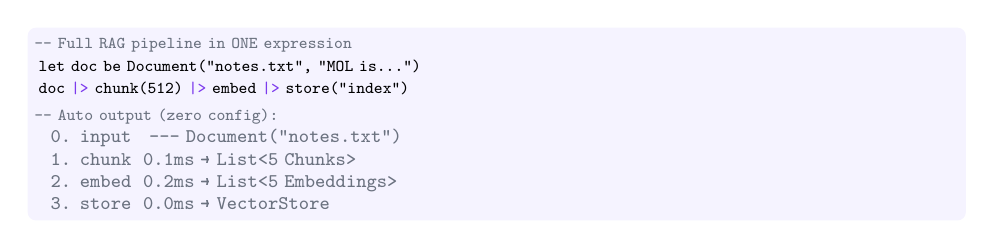
\begin{tikzpicture}
\node[fill=mollight, rounded corners=3pt, inner sep=4pt, text width=\linewidth-14pt, font=\ttfamily\fontsize{6.5}{8}\selectfont] {%
\textcolor{molgray}{-{}- Full RAG pipeline in ONE expression}\\
\textbf{let} doc \textbf{be} Document("notes.txt", "MOL is...")\\
doc \textcolor{molpurple}{\textbf{|>}} chunk(512) \textcolor{molpurple}{\textbf{|>}} embed \textcolor{molpurple}{\textbf{|>}} store("index")\\[2pt]
\textcolor{molgray}{-{}- Auto output (zero config):}\\
\textcolor{molgray}{~~\textrm{\scriptsize\ttfamily 0. input ~~--- Document("notes.txt")}}\\
\textcolor{molgray}{~~\textrm{\scriptsize\ttfamily 1. chunk ~0.1ms \textrightarrow ~List<5 Chunks>}}\\
\textcolor{molgray}{~~\textrm{\scriptsize\ttfamily 2. embed ~0.2ms \textrightarrow ~List<5 Embeddings>}}\\
\textcolor{molgray}{~~\textrm{\scriptsize\ttfamily 3. store ~0.0ms \textrightarrow ~VectorStore}}
};
\end{tikzpicture}

\section{Why MOL?}
\vspace{-0.1em}
{\fontsize{7.5}{9}\selectfont
\renewcommand{\arraystretch}{1.05}
\begin{tabularx}{\linewidth}{@{}l X X@{}}
\toprule
\textbf{Problem} & \textbf{Python/JS} & \textbf{MOL} \\
\midrule
Debugging & \code{print()} & \code{|>} auto-traces \\
Data flow & No pipes & \code{|>} left-to-right \\
AI types & Generic dicts & Native types \\
RAG setup & 50+ lines & One expression \\
Safety & None & \code{guard} + \code{access} \\
\bottomrule
\end{tabularx}
}

\section{Language Syntax}
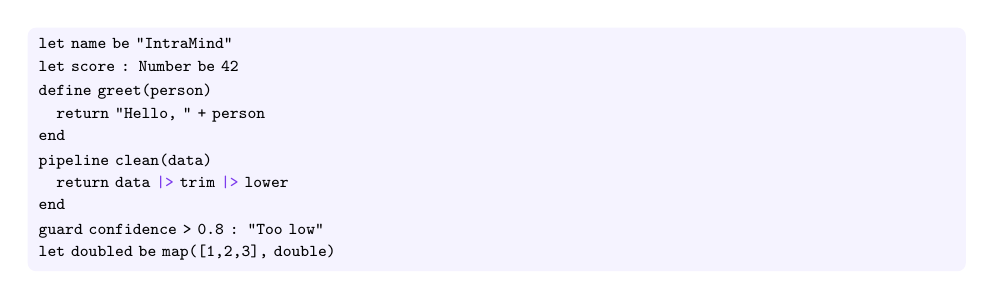
\begin{tikzpicture}
\node[fill=mollight, rounded corners=3pt, inner sep=4pt, text width=\linewidth-14pt, font=\ttfamily\fontsize{6.5}{8}\selectfont] {%
\textbf{let} name \textbf{be} "IntraMind"\\
\textbf{let} score : Number \textbf{be} 42\\[1pt]
\textbf{define} greet(person)\\
\quad \textbf{return} "Hello, " + person\\
\textbf{end}\\[1pt]
\textbf{pipeline} clean(data)\\
\quad \textbf{return} data \textcolor{molpurple}{\textbf{|>}} trim \textcolor{molpurple}{\textbf{|>}} lower\\
\textbf{end}\\[1pt]
\textbf{guard} confidence > 0.8 : "Too low"\\
\textbf{let} doubled \textbf{be} map([1,2,3], double)
};
\end{tikzpicture}

\section{Domain Types}
\vspace{-0.1em}
{\fontsize{7.5}{9}\selectfont
\renewcommand{\arraystretch}{1.0}
\begin{tabularx}{\linewidth}{@{}l l X@{}}
\toprule
\textbf{Type} & \textbf{Cat.} & \textbf{Constructor} \\
\midrule
Thought & Core & \code{Thought("idea", 0.9)} \\
Memory & Core & \code{Memory("key", value)} \\
Node & Core & \code{Node("label", 0.5)} \\
Stream & Core & \code{Stream("feed")} \\
Document & RAG & \code{Document("file", "text")} \\
Chunk & RAG & \code{Chunk("text", 0, "src")} \\
Embedding & RAG & \code{Embedding("text", "model")} \\
VectorStore & RAG & \emph{via} \code{store()} \\
\bottomrule
\end{tabularx}
}

\columnbreak

\section{Standard Library (90+ Functions)}
\vspace{-0.1em}
{\fontsize{7}{8.5}\selectfont
\renewcommand{\arraystretch}{1.0}
\begin{tabularx}{\linewidth}{@{}l X@{}}
\toprule
\textbf{Category} & \textbf{Functions} \\
\midrule
\textbf{General} & len, type\_of, to\_text, to\_number, range, abs, round, sqrt, max, min, sum \\
\textbf{Functional} & map, filter, reduce, flatten, unique, zip, enumerate, find, take, drop, group\_by, every, some \\
\textbf{Math} & floor, ceil, log, sin, cos, tan, pi, e, pow, clamp, lerp \\
\textbf{Statistics} & mean, median, stdev, variance, percentile \\
\textbf{Collections} & sort, sort\_by, sort\_desc, binary\_search, reverse, push, pop, keys, values, contains, join, slice \\
\textbf{Strings} & split, upper, lower, trim, replace, starts\_with, ends\_with, pad\_left, pad\_right, format \\
\textbf{Crypto} & hash, uuid, base64\_encode, base64\_decode \\
\textbf{Random} & random, random\_int, shuffle, sample, choice \\
\textbf{Maps} & merge, pick, omit \\
\textbf{Types} & is\_null, is\_number, is\_text, is\_list, is\_map \\
\textbf{RAG} & chunk, embed, store, retrieve, cosine\_sim, think, recall, classify, summarize \\
\textbf{Debug} & display, tap, inspect, to\_json, from\_json \\
\bottomrule
\end{tabularx}
}

\section{CLI \& Tooling}
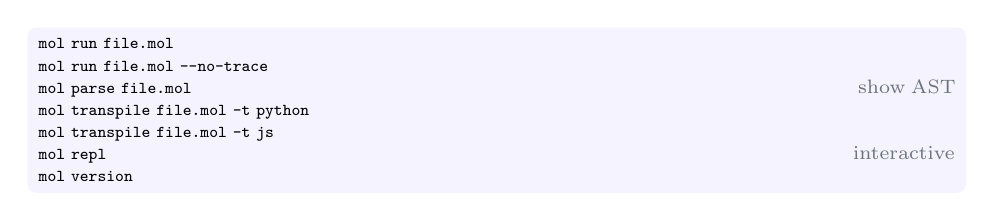
\begin{tikzpicture}
\node[fill=mollight, rounded corners=3pt, inner sep=4pt, text width=\linewidth-14pt, font=\ttfamily\fontsize{6.5}{8}\selectfont] {%
mol run file.mol\\
mol run file.mol -{}-no-trace\\
mol parse file.mol\hfill\textcolor{molgray}{\textrm{\scriptsize show AST}}\\
mol transpile file.mol -t python\\
mol transpile file.mol -t js\\
mol repl\hfill\textcolor{molgray}{\textrm{\scriptsize interactive}}\\
mol version
};
\end{tikzpicture}

{\scriptsize\textbf{VS Code Extension} included --- syntax highlighting, 20+ snippets, code folding for all block structures.}

\section{Version History \& Roadmap}
\vspace{-0.1em}
{\fontsize{7}{8.5}\selectfont
\renewcommand{\arraystretch}{1.0}
\begin{tabularx}{\linewidth}{@{}l l l X@{}}
\toprule
\textbf{Ver.} & \textbf{Date} & \textbf{Status} & \textbf{Highlights} \\
\midrule
0.1.0 & 02-08 & \badge{molgreen}{Done} & Grammar, AST, interpreter, 4 types, CLI \\
0.2.0 & 02-09 & \badge{molgreen}{Done} & \code{|>} auto-trace, guard, RAG types \\
0.3.0 & 02-10 & \badge{molgreen}{Done} & 42 new algorithms, 90+ stdlib \\
0.4.0 & --- & \badge{molorange}{Next} & Sovereign AI, agent blocks \\
0.5.0 & --- & \badge{molgray}{Plan} & Async pipelines, HTTP server \\
1.0.0 & --- & \badge{molblue}{Vision} & Package manager, cloud deploy \\
\bottomrule
\end{tabularx}
}

\end{multicols}

\vspace{0.1em}
\begin{center}
{\small\bfseries\color{moldark} Built for IntraMind by CruxLabx}\quad{\color{molgray}$\cdot$}\quad{\small\color{molgray} Creator: Mounesh Kodi}\quad{\color{molgray}$\cdot$}\quad{\small\color{molgray}\url{github.com/crux-ecosystem/mol-lang}}
\end{center}

\end{document}
